% $Id: $
\documentclass[a4paper,12pt]{report}

% The following makes latex use nicer postscript fonts.
\usepackage{times}
\usepackage[english]{babel}
\usepackage[colorlinks,urlcolor=blue,linkcolor=blue]{hyperref}
\usepackage{wrapfig}

\usepackage{vubtitlepage}
\author{Ayrton Vercruysse}
\title{TIAMAT: A Multi-touch Tablet IDE for AmbientTalk}

%\promotortitle{Promotor/Promotors}
\promotor{Prof. Dr. Wolfgang De Meuter}
\advisors{Dries Harnie\\
          Lode Hoste}
\faculty{Faculty of Science}
\advisortitle{Advisors}
\department{Department of Computer Science\\ and Applied Computer Science}
\reason{}

\date{2012-2013}
          
\begin{document}

\maketitlepage
\tableofcontents
\chapter{Introduction}
\section{Goal}
This document is made to be a guide with the organisation, implementation and evaluation of the TIAMAT project. It will explain choices that have been made concerning the implementation and will evaluate
the relevance of the chosen solution. To illustrate this all the specifications of this project will be listed and we will explain how these are implemented.
Next to a reflection about how we implemented the project we will also provide some context. This being why the project is made, who will be using it and as last we will have a look at some 
related work.
Next to the implementation we will have a social experiment with the application. We will distribute the app to several people and let them test the app. We will evaluate if the app is an 
improvement to the old apps which provide the possibility to create some AmbientTalk programs. 
Thanks to the implementation details the users of the application will be able to use this document as a reference to find what the possibilities of the app are. They can guide a user to use the
app to its fullest potential.

\section{Scope}
The scope of this project is a third bachelor thesis at the Vrije Universiteit Brussel. The 3th bachelor thesis is given at third bachelor students computer sciences. The goal of this bachelor thesis
is to let the bachelor students  participate in some actual research at the university. This has been chosen over giving the students a predefined task.
\section{Definitions and Acronyms}

\begin{tabular}{ l l }
  VUB & Vrije Universiteit Brussel \\
  IDE & Integreted Develepment Enviorment \\
  AST & Abstract Syntax Tree \\
  MANET 	& Mobile Ad-Hoc Network \\
  OHA & Open Handset Alliance \\
  App & Application. Programs on smartphones and tablets \\
  MT4j & Multi-Touch for Java \\
\end{tabular}
\section{Product Placement}
This product is an IDE for AmbientTalk on Android devices. AmbientTalk is a programming language developed to mainly program within Mobile Ad-Hoc networks. MANETs are mostly used to program
for mobile devices like smartphones and tablets. AmbientTalk is developed to be able to handle with possible disconnects within a MANET.

As AmbientTalk programs are made for Android devices one should be able to program on the Android device itself. Currently, on pc's, AmbientTalk is being programmed in Eclipse. There are currently
several apps which port Eclipse to Android. The only drawback is that these are not developed to be really usable on these devices. Most of them even assume that there is a keyboard connected to the
tablet. Other drawbacks are that the screen of the pc version of Eclipse would not fit a much smaller tablet or smartphone screen.   

The goal of this product is to be a useful alternative to program AmbientTalk code on an Android device. We won't make use of the existing technologies of Eclipse but instead we will develop an entire
new technique based on the usage of the internal AST. We will manipulate the AST directly instead of creating a sequence of statements which will be mapped to an AST afterwards.

By manipulating the AST we can make use of predefined templates. This will help to create source code without defining a sequence of statements. For every possible part of an AST
a template is created which can be added to the current AST, making it possible to create an entire program. 
\section{Users}
The goal of the Application is to be able to create programs on the Android devices. As AmbientTalk is a programming language one should have basic knowledge of programming within the AmbientTalk
environment. Without a knowledge of the AmbientTalk language it is not easy to create a sound program.
As AmbientTalk is developed at the university and momentarily is used as an example on different conferences the app can be helpful to create a small example of an AmbientTalk program instead 
of always needing to use a computer.

\section{Used Software}
\subsection{AmbientTalk}
AmbientTalk is a programming language developed at the VUB in 2005. The goal of the language was to focus on making programs within Ad-Hoc networks. This means that AmbientTalk is developed mainly
to create programs on mobile devices. AmbientTalk combines elements from other programming languages such like Scheme (closures), Smalltalk (pure OO), Self (prototypes and delegation) and some
other languages.

AmbientTalk was originally a part of a doctorate study made by Jessie Dedecker. His goal was to create an extension to the already existing programming language Pic\% (pic-oh-oh). Pic\% itself
was an extension of Pico. Pico was developed by professor Theo D'Hondt in 1996. Pico was developed merely to be used with an educational purposes. Pico is being used as a programming language to
illustrate how programming languages are being made.

Pico got it's design principles and concepts from Scheme. The goal of Pico was to be a programming language based on simple rules, easy to extend. Thanks to the simplicity and extendability of Pico
this language is often used to do some research to possible extensions and features for programming languages. This is the reason why a lot of offsprings of Pico are created, all with their own
special attention to certain problems or extensions. When AmbientTalk was being developed special attention was given create distributed programs within ad-hoc networks.
Momentarily AmbientTalk/2 is being used. It's the successor of the original AmbientTalk. Even though AmbientTalk/1 was already successful concerning the programming features for mobile Ad-Hoc
networks it lacked some important features to create bigger software applications, such like exception handling,...

In 2006 Tom Van Cutsem and Stijn Mostinckx started developing AmbientTalk/2, the current version of AmbientTalk. The changes between AbmientTalk/1 and AbmientTalk/2 are quite big. There has been
made an entire new design for most aspects of the language, including the syntax. The reason to change the syntax was to make AmbientTalk more accessible for people who don't have any experience
with Pico. 

AmbientTalk is still mainly used by students at the VUB to do some research. But, slowly but surely, AmbientTalk became a useful, handy programming language which was usable to create some
rather big programs. Because the focus of AmbientTalk lies within the distributed networks and this is still an area in which a lot of research is being done there aren't a lot of good alternatives.
This made AmbientTalk a good alternative to create some real-life software.

The symbiosis with the underlying Java Virtual Machine enables the possibility to use some parts of the Java programming languages within AmbientTalk, which makes it possible to combine both languages within
one project.

The renewing element of AmbientTalk is so big that it became the main subject of the Distributed and Mobile Programming Paradigms course taught at the VUB.
\subsection{Google Android}



\subsubsection{General}
\begin{wrapfigure}{r}{0.5\textwidth}
  \begin{center}
    
\includegraphics[width=0.48\textwidth]{images/android.png}
  \end{center}
  \caption{Android logo}
\end{wrapfigure}
Android is an open source platform for mobile devices, owned by Google. Android is developed by Android Inc., a company bought by Google in 2005, which later placed it 
within the Open Handset Alliance (OHA). 

It's an on Linux based operating system and is mainly programmed in C (core), Java (UI) and C++.

Android is originally created by Android Inc., a company founded by Andy Rubin, Rich Miner, Nick Sears and Chris White in 2003. Their goal was to create an operating system
for " ... smarter mobile devices that are more aware of its owner's location and preferences.`` 

On October 17th 2005 Google bought Android Inc. and made it a part of their company. Even after Google bought the company founders Andy Rubin, Rich Miner and Chris White
kept working for Android. Already back then the goal of Google was to focus on the market of mobile devices with Android.

Only on December 9th 2009, together with the founding of OHA, the first product of Google concerning the market of the mobile devices was announced; Android. An on Linux 
kernel version 2.6 based platform for mobile devices.

According to estimations in the second quarter of 2009 approximately  2.8\% of new smartphones had Android as operating system. In the fourth quarter of 2010 this number
had grown to 33\% what made it the best selling smartphone platform. In the third quarter of 2011 this would already have grown to 52.5\%. In February 2012 Andy Rubin
said that Google activates 850000 smartphones or tablets on a daily basis. 
\begin{figure}
  \centering
    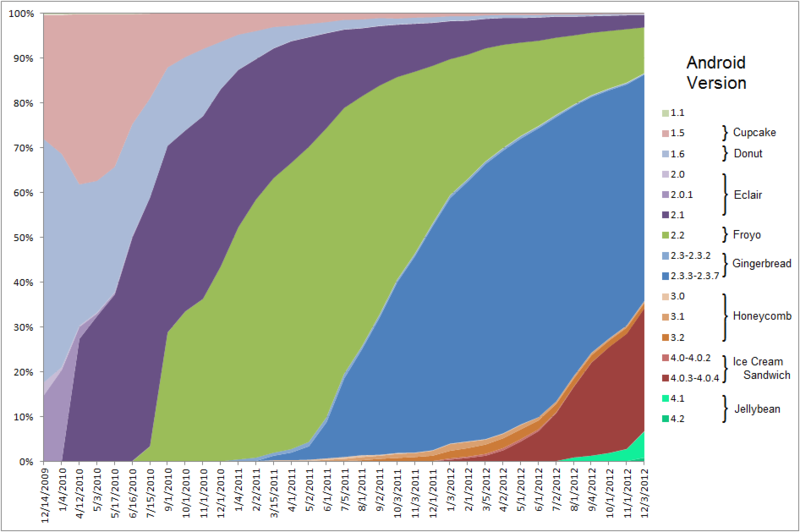
\includegraphics[width=0.99\textwidth]{images/Android_historical_version_distribution.png}
  \caption{Android historical version distribution}
\end{figure}

\subsubsection{Versions}
Through the years multiple versions of Android have been released. In November 2007 a beta version was released, but only on September 23th 2008 Android 1.0 was released.
Android 1.0 was introduced on the HTC Dream. This version was already equipped with the Android Market, an application which gives you the option to download and update
new applications, camera support, synchronization with, and use of, most Google products, like Gmail, Google Calendar, Google Contacts, Google Search, Google Talk,... 
Also Wi-Fi and bluetooth were already supported, just like a Youtube media player.

After Android 1.0 in February 2009 Android 1.1 was released. After Android 1.1 a next version of Android, Android 1.5 which was given the name Cupcake was released followed by 
Android 1.6, called Donut. In October 2009 Android 2.0 got released. It was called Eclair. Eclair was followed by Froyo (2.2.x) and later the popular Gingerbread (2.3.x)
Next to the 2.x series in February 2011 the 3.x (Honeycomb) version got released. This version was created with focus on tablets and no longer on smartphones.

In October 2011 Android 4.0.1 (Ice Cream Sandwich) was presented. ICS was the version of Android which should combine the 2.x series and 3.x series to the 4.x series.
This means that there will be no longer 2 parallel versions of Android, but only one, working on both smartphones and tablets. This made it easier for Google, so they 
didn't need to keep two versions up to date but only one. On July 9th 2012 a new version of the Android 4.x series was released named Jelly Bean (4.1).
In Figure 1.2 one can see a chart showing global Android version distribution from November 2009 to December 2012.

\subsubsection{Design}

Android is based on a Linux kernel, with middleware, libraries and APIs written in C and application software in Java. In Figure 1.3 the architecture of Android is shown.
The top layer of the figure; the Application Layer are the applications which are deployed on the phone when bought, like an SMS program, calendar, internet browser,...
All these applications are written in Java. The application framework is made to create an open developing platform. Android gives developers the possibility to develop
rich and innovative applications, by giving them the liberty to make use of all hardware, like location information, setting alarms, add notifications to the status bar,...

The libraries layer contains a number of C/C++ libraries which are being used in multiple layers of the Android system. Developers are able to explore these libraries
trough the Android Application framework for developers. Some of these libraries are SGL (an underlaying 2D engine), FreeType (a bitmap and vector renderer), MQLite (a 
database engine),... The Android Runtime part is a number of core libraries which gives most Java functionalities. Last there is the Linux kernel which provides safety, memory
management, process management, network stacking and driver models. It also functions as abstraction layer between the hardware and the rest of the software.
\begin{figure}
  \centering
    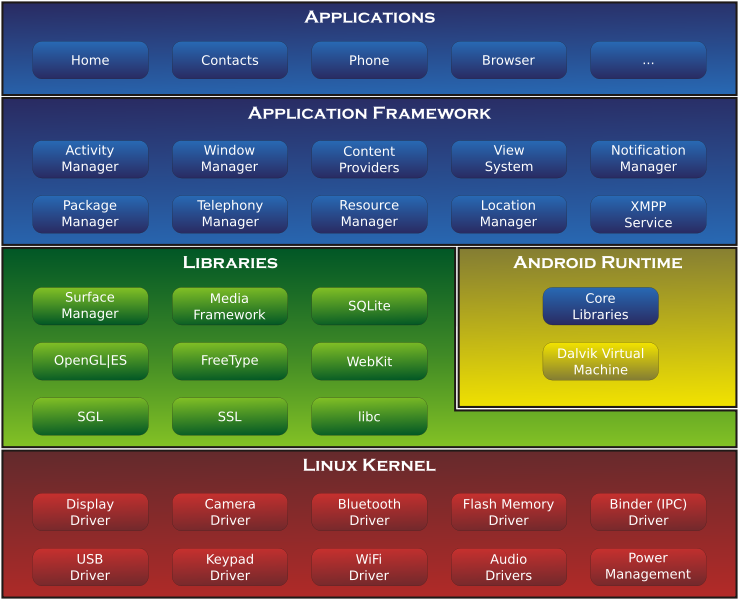
\includegraphics[width=0.99\textwidth]{images/Android-System-Architecture.png}
  \caption{Android System Architecture}
\end{figure}
\subsubsection{Open Handset Alliance}
The Open Handset Alliance (OHA) is a consortium of 84 firms to develop open standards for mobile devices. Practically this translates in promoting Android. OHA is founded
on November 5th 2007, with as main founding company Google, together with 34 other firms. These firms are active in creating software, creating mobile devices or creating
chips. The main goal was to make Android a worthy competitor of other mobile platforms like those developed by Apple, Microsoft, Nokia (Symbian), HP, Research in Motion 
and Barda.

Some of the companies who aided founding OHA were, besides Google, HTC, Sony, Dell, Motorola, Qualcomm, Texas Instruments, Samsung Electronics, LG Electronics, T-Mobile,
Nvidea,... 
\subsection{MT4j}
\subsubsection{General}
Multi-Touch for Java is developed to make it possible to create multi touch applications within the Java programming language. It's an open source Java Framework. It offers a GUI in which we can use
shapes like rectangles, rounded rectangles, ellipses, polygons,... To each of these forms gestures can be attached. These can be in 2D or 3D. Next to the predefined shapes you can also make use 
of buttons, text areas, sliders and a multi touch keyboard.
\subsubsection{Architecture}
The architecture of MT4j is built in multiple layers which communicate with each other. Using event messages which are sent from one layer to another. The different layers within MT4j are the 
Presentation Layer, Input Processing Layer, Input Hardware Abstraction Layer and the Input Hardware Layer.
\begin{figure}
  \centering
    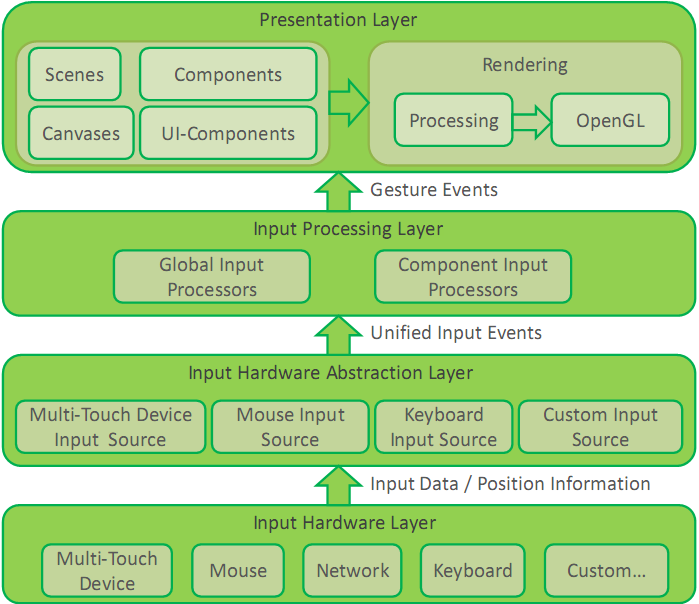
\includegraphics[width=0.99\textwidth]{images/ArchitectureOverview2.png}
  \caption{MT4j Architecture}
\end{figure}
\\
\\
\textbf{Input Hardware Layer}
\\
By making use of the Input Hardware Abstraction Layer MT4j can give support to different kinds of input hardware, while only little alternations are needed within the Hardware Abstraction Layer.
Within this layer all raw input gets reformed to unified input events. The only change needed when one wants to use a new form of input is to change the abstract superclass of all input sources
and the specific input for this new part of hardware.
MT4j already has a number of input methods which are supported, like a keyboard, mouse,... All input methods can be used synchronously and together without chances on conflicts.
\\
\\
\textbf{Input Processing Layer}
\\
In MT4j the input processor gets used on two moments within the input event flow. The first moment is when input directly from the Input Hardware Abstraction Layers comes, the other moment
is at the component level. This means one can recognize gestures which are meant for only one component.
\\
\\
\textbf{Presentation Layer}
\\
The Presentation Layer within MT4j uses scenes. Scenes are made to be able to separate different aspects of a program, input and output, in a nice clean encapsulated 
manner. An example of multiple scenes could be a game where there's one scene to create the menu and an other scene in which the actual game is played.

Next to scenes MT4j also uses components. Components are parts of a program which can be connected in a hierarchical manner. So one can use a basic component and add multiple
components within this component. Here we can see as the basic component the background of the application, and within this component one or more other components are used.

The most basic component of MT4j is a canvas. A canvas is the link between multiple components and the input of the hardware. It can check what other components are on
what place within the screen at a given time.

To render the MT4j components they use the Processing toolkit. Processing is an open source toolkit that is used to create data visualization and interaction.

\subsubsection{MT4Android}
MT4Android is an Android version of MT4j. Because MT4j lays the focus on multi touch and is made within Java it seemed a logical step to port MT4j to the Google Android 
platform. MT4Android is made by a coworker of MT4j. MT4Android still isn't a full version, but there is a beta version available.


\chapter{Implementation Status}
\section{ASTs}
\subsection{Making ASTs}
\textbf{Description: } Every piece of code used in the IDE will be directly linked to an AST. For this matter there has to be a possibility to create new ASTs from scratch.
To create new ASTs we will need to implement the different parts of which an AST can exist. These different parts of an AST will be called a Nodes. We will start with
a list of possible nodes with which basic programs can be made. Later extra kinds of nodes can be added to the AST.
A superclass Node will be implemented which will organize the tree structure by providing operations like getParent(), which gets the parent of a Node, setChild(oldChild, newChild)
which will set a child of a node and getChilderen() to get the children of a Node. By using these operations new trees can be created. 
The types of nodes that will be implemented are: Placeholder, Begin, Block, Definition, Value, Argument List, Function, Function Call, Function Definition, Operation, Table, Table Call
Table Definition.
 \newline
\textbf{Priority:} High \newline
\textbf{Status: }  Within the vub.ast package the implementation of the Nodes can be found.   \newline
\subsection{Deleting ASTs}
\textbf{Description: }When we have an excising AST and parts of this AST became irrelevant there should be a possibility to remove this AST. The removing of an AST, in total,
or only a part of an AST will happen by replacing this AST by the Placeholder node. This possibility will be, as said in 1.1 implemented in the Node class, by means of the 
setChild(oldChild, newChild) function. \newline
\textbf{Priority:} High \newline
\textbf{Status: } The possibility to set children of nodes of implemented in each node. This means that we can delete nodes by setting the 
node we want to delete to null in the parent node.\newline
\subsection{Replacing parts of ASTs}
\textbf{Description: }When new Nodes will be created it's children, if there are any, will be made by Placeholders. When making a function for example, we'll implement the operation,
but the two operands will be initialized with a Placeholder node. To be able to change these Placeholders to more relevant Nodes we should be able to 
replace existing Nodes by other Nodes, in this example maybe a Value, or an other Operation. This can be done on a similar way as the deletion of ASTs, by making use of the replaceChild(oldChild, newChild) method.\newline
\textbf{Priority:} High \newline
\textbf{Status: } In the same way of deleting ASTs replacing parts of an AST can be done. We just set the child we want to change to the 
new node. These possibilities are implemented the Node class.\newline
\subsection{Rendering ASTs to text}
\textbf{Description: } To be able to pass the constructed code to the AmbientTalk interpreter we have to convert the AST to an understandable format for the interpreter. The 
interpreter works with a text file containing AmbientTalk code. This means that the ASTs have to be converted to text. Converting an
AST to a text should be a function within each Node, calling the same function recursively on all of it's children.\newline
\textbf{Priority:} High \newline
\textbf{Status: } Every node can be rendered to text. There's a function foreseen in every subclass of the Node class, called toString(). 
Each of these call the toString() function on it's children as well.\newline
\section{Templates} 
\subsection{Templates creating ASTs}
\textbf{Description: } For convenience we will make use of templates. Templates will be frequently used parts of code that will be saved. The way templates will be stored in the 
memory will be by an AST. Every time a template is used withing the program a copy of this AST will be made and inserted into our current program.
These templates can be frequently used functions, but mainly these will be the ASTs representing basic elements of the language like the if-then-else structure, when-discovered,...\newline
\textbf{Priority:} High \newline
\textbf{Status: }There is a file called 'templates.xml' containing all templates that we currently use. Within the TemplateReader class these templates are being read and translated to ASTs. \newline
\subsection{Creating templates from XML}
\textbf{Description: } To keep a clear view on what template functions we have, and make it easy for users to add templates, without having to know the implementation
of the entire program we will keep the Templates in a separate XML file. When having an XML file containing the structure to create new Templates a function will be implemented that creates, from the XML file, a new AST, which 
can be used as a Template within the program.\newline
\textbf{Priority:} High \newline
\textbf{Status: }There is a file called 'templates.xml' containing all templates that we currently use. Within the TemplateReader class these templates are being read and translated to ASTs. \newline
\subsection{Create templates from functions}
\textbf{Description: } When a newly created function is often used by the user and he wants to save this function, the possibility to write this function, in correct XML, to
the existing XML file will be provided. This means that whenever the program is terminated functions can be stored inside the XML file.\newline
\textbf{Priority:} Low \newline
\textbf{Status: } Every new function that is being created is saved as a template within the program. As every node has the possibility to be translated to XML it is fairly easy to add the option to write this XML to 
an XML file.\newline
\section{Interface}
\subsection{Rendering of nodes}
\textbf{Description: }Each type of node has to have a screen representation. For each node we need a function that displays the Node on the screen, and 
that recursively calls the display function of all children of this node. We won't implement these displays within the separate types of nodes, discribed in 1.1, but 
for each node we will implement a separate display function. This with as goal that we can re-use our AST implementation without having to dead
with the program specific display possibilities.  \newline
\textbf{Priority:} High \newline
\textbf{Status: } Within the vub.ast.Renndering package all needs to render a node to the screen is kept. \newline
\subsection{Lay-out engine}
\textbf{Description: } We will make a render manager, this manager will render all nodes and make sure they are organized on a ordered way. The render manager will use
indention to organize nodes across the screen.
\textbf{Priority:} High \newline
\textbf{Status: } Within the vub.rendering package we have the RenderManager class. This class gives you the possibility to render nodes
by sending MTRectangles to them, and tell the class how to render them. This being next to the previous node or under the previous node. 
The is also to option to indent the next function. This for when one want to show a new node under the previous one, but indented. \newline
\subsection{Creating functions on the spot}
\textbf{Description: } Whenever a new function (or variable) is created within the program a link to call this function will be added to the menu's. This means that we can
easily re-use a made variable or have an easy way to call an earlier created function. \newline
\textbf{Priority:} High \newline
\textbf{Status: } Newly created functions will have a automatically have a functionCall made. This will be added to the list of possible
functioncalls.\newline
\subsection{Buttons}
\subsubsection{Menu's}
\textbf{Description: } To keep track of all templates or calls that can be made we will need a menu that gives us the possibility to insert templates in to the code.
We will use one a menu with some sub menu's, divided for each kind of templates. These can be provided functions self implemented function, used variables,... \newline
\textbf{Priority:} High \newline
\textbf{Status: } In the package vub.menus all menus that are availeble in the program are implemented. These are a standard menu, a menu for functions, operations, own functions, definitions, variables, ...\newline
\subsubsection{Run button}
\textbf{Description: } Thanks to requirements 4.2 we can evaluate made code with an external AmbientTalk app. To do this we'll add a button
to the main screen which will first make sure requirement 1.4 is done, the creation of a text file with the current code, and later on run the AmbientTalk app, as described in requirement 4.2.
\textbf{Priority:} High \newline
\textbf{Status: } The implementation of this button can be found in the Tiamat class within the vub.tiamat package.\newline
\subsubsection{Delete button}
\textbf{Description: } To be able to delete some code, as described in 1.2 we need a way to select what code will be deleted. This is why we will
implement a delete button on the screen, which deletes the current selected piece of code. This can be done by pressing this button or by dragging the selected code to this place. 
\textbf{Priority:} High \newline
\textbf{Status: } The implementation of this button can be found in the Tiamat class within the vub.tiamat package. \newline
\subsection{Views}
\subsubsection{Colorcoding keywords}
\textbf{Description: }As in many languages the use of color coding should be done here aswell. We  will try to achieve the same color coding as
being used in the official AmbientTalk IDE in Eclipse. \newline
\textbf{Priority:} Low \newline
\textbf{Status: } The implementation of MT4j does not allow us to make use of color coding. Because of a bug within the code it is impossible
to change the color of only 1 word. This is on the other not the problem when one to change the background color of a MTTextArea. \newline
\subsubsection{Colorcoding types}
\textbf{Description: } Next to the color coding of keywords we will implement color coding on the types of words. This means that we will give
Placeholders different colors, just like VariableNames,... \newline
\textbf{Priority:} Low \newline
\textbf{Status: } Unlike the color coding of keywords the background color of MTTextAreas can be edited.\newline
\subsubsection{Codefolding}
\textbf{Description: }The use of AST should gives us the possibility to easily fold in certain parts (read piece of the AST) of our code. This can be done by just not
rendering certain nodes, and it's children, of the AST. \newline
\textbf{Priority:} Low \newline
\textbf{Status: } \newline
\subsubsection{Move code}
\textbf{Description: } By using the possibility of deleting parts of ASTs and saving parts of ASTs a copy-pasty system, or even moving of code to places that make sense belongs
to the possibilities.\newline
\textbf{Priority:} Low \newline
\textbf{Status: } \newline
\subsection{Gestures}
\subsubsection{Selection of code}
\textbf{Description: } To be able to replace, delete, move,... code we need a possibility to select certain parts of the code. This will be done
by a tap or doubletap gesture. The selected code will be marked and it will be possible to makes changes to this code.\newline
\textbf{Priority:} High \newline
\textbf{Status: } Code can be selected by a simple tap on top of it. The selected code will be surrounded by a red square to indicate it has been selected. \newline
\subsubsection{Pinch-to-zoom}
\textbf{Description: }When starting on a piece of code by using the pinch-to-zoom function the selected part of code should be extended. This can be done by enlarging the selected
area from the current AST to the parent of this AST. \newline
\textbf{Priority:} Low \newline
\textbf{Status: } By zooming on a certain piece of code more parts of the code will be selected.\newline
\subsubsection{90° degrees turning for comments}
\textbf{Description: }When a piece of code is selected, and afterwards this piece of code gets turned around for 90 degrees, this piece of code should be commented out. 
Commented code should not be written to the text file when this is called on this AST. \newline
\textbf{Priority:} Low \newline
\textbf{Status: } By turning the screen 90° code will be commented out.\newline
\subsubsection{Fast scrolldown}
\textbf{Description: }When we want to scroll down a longer piece of code we can use the scroll with two fingers gestures to get us scroll faster. \newline
\textbf{Priority:} Low \newline
\textbf{Status: } By scrolling over the code with 2 fingers you can scroll down the code.\newline
\section{Evaluating code}
\subsection{Writing code to text file}
\textbf{Description: }To make use of the AmbientTalk app we need a text file with the AmbientTalk code. We can make use of the toText() function of each node to translate our
current AST to plain text, and afterwards we will need to write this text, into a text file.  \newline
\textbf{Priority:} High \newline
\textbf{Status: } The function to write the code to a file can be found inside the action of the run button in the Tiamat class. Also the outputstream used for this can be found in this class.\newline
\subsection{Call external AmbientTalk app}
\textbf{Description: }The external AmbientTalk app, which makes use of the text file from the previous - insert number- should be called. To get this app called we will implement
a button on the screen, which first gets the text file created and afterwards calls the AmbientTalk app. \newline
\textbf{Priority:} High \newline
\textbf{Status: } \newline
\subsection{Return to TIAMAt after evaluating code}
\textbf{Description: } The AmbientTalk app will evaluate the program. After the evaluation of this program and returning the result we should get back the our application to
create the possibility to edit our current program\newline
\textbf{Priority:} High \newline
\textbf{Status: } \newline
\section{Advanced Interactions}
\subsection{Extra interface for comments}
\textbf{Description: } An extra interface can be created in which we can store extra comments. This interface should only be called on object which could get any use of extra comments.
 \newline
\textbf{Priority:} Low \newline
\textbf{Status: } There is an extra interface for comments implemented, but currently not in use.\newline
\subsection{Speaking comments}
\textbf{Description: } A nice feature is to add spoken comments to our program. The possibility to add spoken comments will be integrated in the
extra interface for spoken comments, announced in requirement 5.1. There will be added extra buttons to record comments and play these comments.\newline
\textbf{Priority:} Low \newline
\textbf{Status: } \newline
\subsection{Selector for Java classes}
\textbf{Description: } Within the AmbientTalk language it's possible to make use of a Java class selector. Adding this feature to this implementation
will make sure that our project becomes a better alternative to the pc one.\newline
\textbf{Priority:} Low \newline
\textbf{Status: } \newline
\subsection{Multiple tabs}
\textbf{Description: } If we want to make bigger programs it would be easy to be able to have multiple tabs. Certainly when big programs exist of multiple files. To make this possible we would need
to save multiple AST trees and implement a possibility to switch between the different tabs.\newline
\textbf{Priority:} Low \newline
\textbf{Status: }
\subsection{Saving files}
\textbf{Description: } As we will implement a write to XML to save new Template into an XML file we could use this procedure to save an entire program in XML, and later rebuild our AST and on this way 
reconstruct our program. \newline
\textbf{Priority:} Low \newline
\textbf{Status: } Every Node has the possibilty to show it's own XML representation. This representation can be saved by clicking the save button. Whenever the app starts again there will be asked if you want to open
previously stored code.


\chapter{Related work}
\section{TouchDevelop}
TouchDevelop is a programming environment made for Windows phones. TouchDevelop allows you to create some simple applications for your phone and add these later to the Windows Phone Marketplace. 
Because TouchDevelop is made to create applications for the device on which they are developed they can make use of really powerful templates. TouchDevelop offers you the possibility to make use 
of most of the built in sensors and files upon your device, such like media files, web cloud, network, gps,... This makes it possible to develop apps which only react when one shakes the phone or
only when the phone is faced up or down.

TouchDevelop is meant for students and people who like to program in their free time, and not for professional developers. It makes the making of own applications so easy that everyone with a 
basic knowledge of programming can start making his own applications. Different than with TIAMAT these applications are being made within an entire new programming language. This language
is made from scratch to work with Windows Phones, while AmbientTalk was developed to work on plural platforms.

The goal of TouchDevelop was not to be and IDE for an existing programming language, like TIAMAT, but to develop an entire way to create some application on the device for which the application
is meant to run.  

\section{CodeToGo}
The best known app to create programs on tablets is called CodeToGo. CodeToGo is an app created for iPhone which makes you able to program
for a wide vary of languages, like C, C++, Clojure, Erlang, Fortran, Haskell Java, PHP, Ruby, Scheme... For each of these languages a built in HelloWorld example. This gives you a good idea of how
you can create new programs with these languages. It looks like it is a good IDE for programmers, with guidance for people who want to learn new languages. On the downside it is not really
made for tablets and phones. The idea behind this IDE is that you can write, save and load code. This brings us to a second downside of CodeToGo, you can't run the code on your iPhone/iPad. If you
want to run your code you must have an internet connection.

Additionally on the website of CodeToGo there is a connnection to Dropbox you can use. You can save code from your iPod/iPad straigth to Dropbox, or go the other way around and save files
from your computer to Dropbox and open them in CodeToGo.

To ease up the use of the keyboard of the iPhone/iPad the creators of CodeToGo made their own keyboard. This keyboard has an extra row of commonly used keys added to the default keyboard. 
You can customize this extra row of keyboard for every language you are programming in.
\begin{figure}
  \centering
    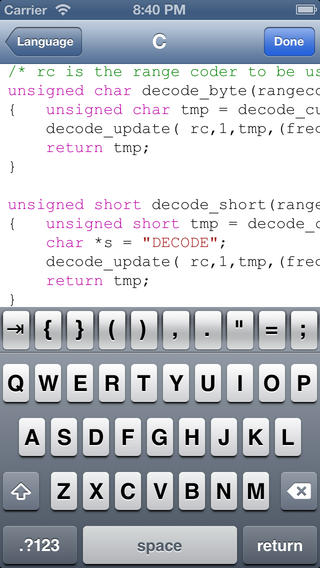
\includegraphics[width=0.40\textwidth]{images/codetogo1.jpeg}
     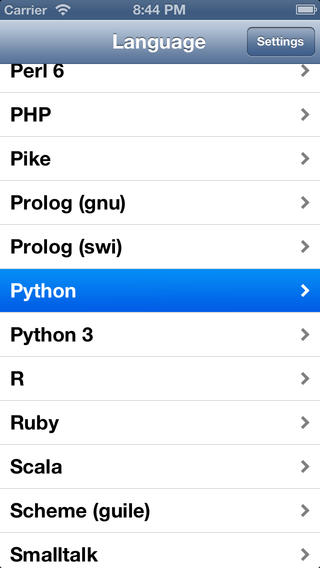
\includegraphics[width=0.40\textwidth]{images/codetogo2.jpeg}
  \caption{CodeToGo}
\end{figure}


\section{Lisping}
Lisping is a program formally known as Touch Scheme. Touch Scheme was developed by a programmer who wanted to program during his vacation on his iPad. To be able to do so he developed an app. 
His main idea was to edit the parse tree within the app.

The huge success of Touch Scheme resulted in a more mature program called Lisping. Lisping is an app which makes you able to write Scheme and Clojure on you iPad. For the same reason as with Tiamat, 
the unability of tablets to easy change text, they here chose to edit your code via the parse tree. ``Rather than manipulting ranges of characters Lisping focusses on selecting, creating and moving 
syntax elements''. This sentence from the Lisping website could come straigth from a Tiamat website. The idea behind both apps are clearly the same.

Some differences between Lisping and Tiamat is that with Lisping they don't use templates as frequent as Tiamat. The goal of Tiamat is to make the user able to built an entire programe with even touching the 
keyboard. If you want the create a function then you click on the create function template within Tiamat, in Lisping you need to start typing (define.... 
\begin{figure}
  \centering
    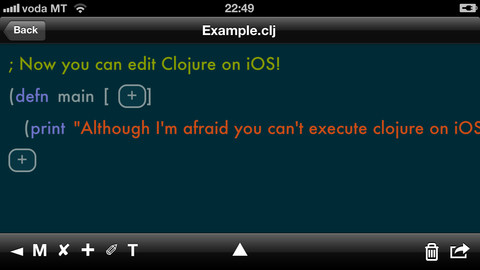
\includegraphics[width=0.75\textwidth]{images/lisping1.jpg}
  \caption{Lisping}
\end{figure}

\section{Editing Haskell as AST rather than text}
Christopher Done has created 'A concept for editing Haskell as an AST rather than text'. This works in a similar way as Tiamat. The idea here is to change certain parts of the AST to the piece of 
code we want. In the video made by Chistopher Done you can see how he edits his Haskell program by clicking on the places where new parts of the code should come. He fills in the parts of the AST
by clicking on them and choosing from a list (of templates) what should be entered on this spot.
This idea is very similar to TIAMAT where we work with Placeholders which can be replaced with actual nodes within the AST of the program.

Christopher Done self says about this idea: ``The idea is that you can't create a syntactically invalid tree, and at each point it can offer you a choice between the valid choices. That's one part, 
the correctness. But that's merely a nice side-effect to the idea of purely syntactical editing, rather than textual editing, so that jumping around, transposing, moving, deleting expressions will 
be a lot easier. Even so that there is no need to care about indentation, but rather moving things about the AST. Still merely a concept at this point. It can technically be generalized to any programming 
language, but Haskell is my main working language so I am targeting it specifically.''
\chapter{Status}
\section{Progress}
In September we started with a part of the project allready. In this section we will explain what progress is made since then. To do so we`ll make use of the requirements on which progress has been made.
\subsection{Lay-out engine}
Big parts of the lay-out engine have been created by now. Even though some serious debugging and readding features from the previous way of displaying stuff need to be added. As an example we can take
the selecting of code. Without the lay-out engine the selected code gets annotated with a red square around it, this has not yet been added to the new lay-out engine.
\subsection{Creating templates from XML}
A major part of the intelligence to create templates from XML has been made, along with the XML file for the most common templates. This needs some extra features to be more dynamic.
\subsection{Extra gestures}
Gestures like 90° turning to comment text have been added, even though these have some bugs, as the program does not registrate the degrees of turning correctly.
After moving code the code returns to its original position when no useful move has been made.
\subsection{Writing code to text file}
The basics of writing a string to a text file on the Android device has been implemented. Every node has it's own way to translate it to text. All of these are implemented in the vub.ast package.

\subsection{Extra changes}
During the changes made in described in the previous sections some extra changes can be made. This could be changes to the lay-out in general,like changing the colors that are being used now, or using the Android 
back button in stead of the one we created ourselves.

\chapter*{Bibliography}
[1]  http://www.mt4j.org/ \newline
[2]  http://en.wikipedia.org/wiki/Android\_(operating\_system) \newline
[3]  http://developer.android.com/index.html \newline
[4]  https://www.touchdevelop.com/ \newline
[5]  http://slidetocode.com/ \newline
[6]  http://soft.vub.ac.be/amop/ \newline
[7]  http://en.wikipedia.org/wiki/AmbientTalk \newline
[8]  Higher-Order Abstract Syntax, Frank Pfenning \& Conal Elliot, Carnegie Mellon University \newline
[9]  Using MetaML: a Staged Programming Language, Tim sheard \newline
[10] Type Extension and Efficient AST Manipulation, K John Goiugh \& Diane Corney \newline


\end{document}

